\chapter{Conversational Search Assistant}
\label{chapter:ConversationalSearchAssistant}


The EHDEN Portal is a web-based platform that facilitates access to information, resources, and tools for data partners, researchers, and other stakeholders involved in the EHDEN project. The portal fosters collaboration, knowledge exchange, and innovation among diverse partners, providing a user-friendly interface to access standardized healthcare data and related resources. EHDEN delivers a catalogue of medical databases across Europe, offering researchers a centralized platform to explore available medical data sources. However, with the increasing number of databases in the catalogue, EHDEN built a tool named Network Dashboards\footnote{\url{https://github.com/EHDEN/NetworkDashboards}} to help researchers to choose the best databases across the catalogue. EHDEN Network Dashboards is a complementary tool of this ecosystem that provides statistical and aggregated information about the databases available on the network. 

However, the catalogue's growth is inevitable, making it difficult and time-consuming for a researcher to find his databases of interest. The proposed solution is to build a conversational search tool for the EHDEN catalogue.

This section describes how the EHDEN Catalogue search assistant and its components were implemented and the decisions and steps made over time.

% falar aqui do LLM e as suas especificações
% vamos falar sobre os dados, information retrieval, LLM e frameworks

\section{Data}
\label{data}
% sao os dados que usaste
% o artigo do cbms CAT
% tudo o que é relacionado com dados

This section details the structure and contents of the data used in the project, explaining their content, and illustrating how they interconnect to provide a comprehensive overview of the databases in the EHDEN network. The data used for this project is the real EHDEN data from the catalogue and the Network Dashboards. IEETA, a partner of EHDEN, provides this data.

There are four main files that contain the data necessary to obtain an overview of the databases available in the EHDEN network: the countries file, the data sources file, the medical concepts file, and the Achilles Results file. It is essential to understand the content of each file and the relationships between their data, as illustrated in Figure \ref{fig_data_diagram}.

To comprehend the purpose of the four files, each is detailed with fields, description and an example of entries. When the data is private and sensitive, not-real examples are included to better understand the content and connections between files.


\paragraph{Countries file {\small\normalfont(\texttt{countries.csv})}}

\begin{itemize}
    \item \textbf{Fields:} \texttt{id}, \texttt{country}, \texttt{continent}.
    \item \textbf{Description:} This file contains of real-world data, listing countries and their corresponding continents. It is used to provide geographical context for the analyses, and supporting studies that require demographic segmentation.
    \item \textbf{Example Entries:}
    \begin{itemize}
        \item \texttt{233, Ukraine, Europe}
        \item \texttt{149, Montenegro, Europe}
    \end{itemize}
\end{itemize}


\paragraph{Data sources file {\small\normalfont(\texttt{data\_sources.csv})}}

\begin{itemize}
    \item {\raggedright\textbf{Fields:} \texttt{id}, \texttt{name}, \texttt{acronym}, \texttt{hash}, \texttt{release\_date}, \texttt{country\_id}.\par}
    \item \textbf{Description:} This file includes essential details of the databases such as the source identification, the database name and the hash code of the EHDEN catalogue.
    \item \textbf{Example Entries:}
    \begin{itemize}
        \item \texttt{1, MEDIBASE, Medical Database for Health Information Exchange, <hash>, NA,107}
        \item \texttt{2, GRAVITAS, Global Repository of Advanced Vaccine Innovations Technologies and Strategies, <hash>, NA, 228}
    \end{itemize}
\end{itemize}

\paragraph{Medical concepts file {\small\normalfont(\texttt{concepts.csv})}}

\begin{itemize}
    \item {\raggedright\textbf{Relevant fields:}
    \texttt{concept\_id}, \texttt{concept\_name}, \texttt{domain\_id}, \texttt{vocabulary\_id}.\par}
    \item \textbf{Description:} The concepts file contains metadata on medical concepts, extracted from OHDSI Athena\footnote{\url{https://athena.ohdsi.org/}}.
    \item \textbf{Example Entries:}
    \begin{itemize}
        \item \texttt{2966436, Latanoprost (Apotex) 0.005\% Eye Drops 2.5 Ml Bottle, Drug, AMT, Containered Pack, NA, 1009551000168106, 2016-11-01, 2099-12-31, NA}
        \item \texttt{2966944, Letrozole (Apotex) 2.5 Mg Tablet, Drug, AMT, Trade Product Unit, NA, 1009571000168102, 2016-11-01, 2099-12-31, NA}
    \end{itemize}
\end{itemize}

\paragraph{Database summaries {\small\normalfont(\texttt{achilles\_results.csv})}}

\begin{itemize}
    \item {\raggedright\textbf{Relevant fields:} \texttt{data\_source\_id}, \texttt{analysis\_id}, \texttt{stratum\_n (from 1 to 5)}, \texttt{count\_value}, \texttt{statistical information}.\par}
    \item \textbf{Description:} Metadata summary of metadata present in the databases providing aggregated analytics. The “stratum\_1” field points to the concept ID. 
    \item \textbf{Example Entries:}
    \begin{itemize}
        \item \texttt{143, 1, NA, 8507.0, NA, NA, NA,988296, NA, NA, NA, NA, NA, NA, NA, NA, NA}
        \item \texttt{138, 2, 8532.0, 8532.0, NA, NA, NA, 1354216, 526.0, 52600.0, 26300.0, 52.6, 25774.0, 52.6, 157.79, 368.2, 499.7}
    \end{itemize}
\end{itemize}

\hspace{1cm}

The combination of these four files gives the necessary information about the databases. Each row of the Achilles Results file contains statistical information about each concept available in the database, and a set of characteristics that are commonly used to filter databases in a cohort study. For instance, the number of samples segregated by range of age. The Figure \ref{fig_data_diagram} shows how these files content are joined.


\begin{figure}[ht]
    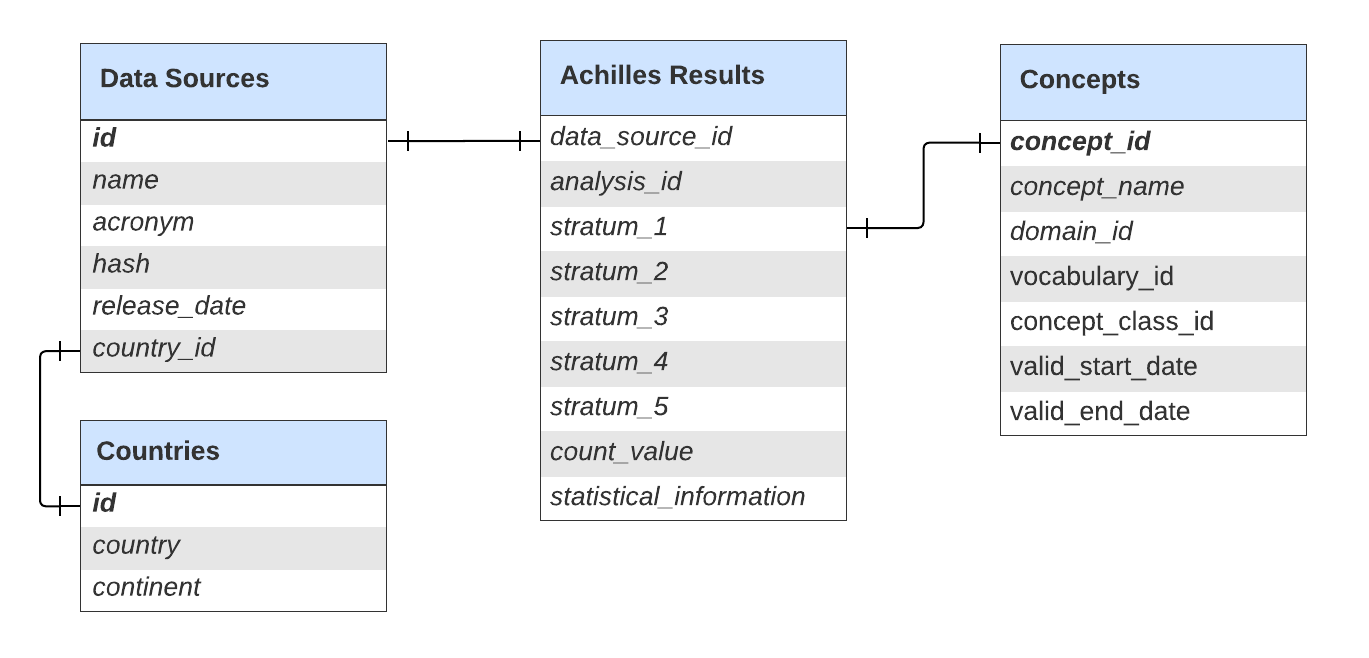
\includegraphics[width=1\textwidth]{figs/chapter3/data_diagram.png}
    \centering
    \caption{The diagram of the connection between the data files.}
    \label{fig_data_diagram}
\end{figure}


\section{Information Retrieval}

After understanding the data and its connections, an IR component is crucial to this project to find the most suitable databases. This section discusses mainly the IR methods tested, the process of indexing and seaching in the collection and an API-driven approach of the IR component.

% tbd


\subsection{BioASQ Challenge 2024}

BioASQ\footnote{\url{http://bioasq.org/}} addresses the information access problem for biomedical experts by organizing challenges in biomedical semantic indexing and question answering (QA). These challenges cover tasks such as hierarchical text classification, machine learning, information retrieval, QA from texts and structured data, and multi-document summarization.

The BioASQ includes several challenges. The IEETA team was involved in 'BioASQ Task 12b', focusing on biomedical semantic QA, including IR, QA, and summarization. This challenge aims to advance the development of systems capable of understanding and answering biomedical questions. Participants must respond to test questions using various types of information, including relevant concepts, articles, and snippets. The challenge involves 5,000 training questions with gold-standard answers and introduces 500 new test questions, all constructed by European biomedical experts. The challenge consists of two phases, A and B:

\begin{itemize}
    \item \textbf{Phase A}: Participants respond to released questions with relevant articles and snippets.
    \item \textbf{Phase B}: Participants provide exact and ideal answers based on questions and provide relevant articles and snippets.
\end{itemize}

To choose and validate the IR method for this project, I joined the IEETA team and was involved in the 2024 edition of the BioASQ challenge. My task was implementing and testing some IR methods to determine which performs better. This task allowed me to have more concrete results. The techniques used and tested were BM25, SPLADE, and BGE-M3. BM25 has already been explained, so here's a brief overview of the other methods tested.


\subsubsection{SPLADE} 

SPLADE\footnote{\url{https://github.com/naver/splade}} is a neural retrieval model that learns query/document sparse expansion through the BERT MLM head and sparse regularization. This technique belongs to Learned Sparse Retrieval because it combines elements of traditional sparse retrieval techniques with machine learning, particularly deep learning. This method can improve the relevance and accuracy of the search results, particularly in complex queries where understanding the context and the semantic relationships between terms is essential.

% tbd

\subsubsection{BGE-M3}

BGE-M3\footnote{\url{https://github.com/FlagOpen/FlagEmbedding/tree/master/FlagEmbedding/BGE_M3 }} is a multifunctional technique because it can simultaneously perform an embedding model's three standard retrieval functionalities: dense retrieval, multi-vector retrieval, and sparse retrieval.

% tbd


\subsection{BM25 Implementation}
\label{bm25implementation}

Although we have tested various methods, the implementation of BM25 has shown promising results. So, BM25 is the selected method for implementing the IR component in this project. The technique was implemented using the PyTerrier PISA, a python interface to PISA\footnote{\url{https://github.com/terrierteam/pyterrier_pisa}}.

This section explains the implementation of BM25, the process of creating documents based on the EHDEN data, and the indexing and searching of these documents.


\subsubsection{Database Indexing Process}

% The data that is used in the IR component is extracted from the EHDEN Network Dashboard database. These data were uploaded by each data owner using CSV files that were generated using automatized profiling tools when executed in the databases. 

% The EHDEN Network Dashboards aggregate all this information in a single structure that was designed to create and maintain an up-to-date collection of databases. Upon the upload of a new file, to update an existing database, or to create a new one, the system initiates a sequence of operations. These not only refresh the central repository but also update the IR component used in the chatbot. 

The IR component must index a collection of documents that thoroughly represent all the concepts within the databases, ensuring a clear understanding of what each database encompasses. To achive this, the data mentioned in the section \ref{data} is used to create the documents.

Figure \ref{fig_struct} represents the different stages of the data. The first part of the figure, A), represents the three data files detailed in the section \ref{data}. \hl{These are received from the EHDEN Network Dashboard.} One contains information about the data sources, another contains the metadata summary of the databases (Achilles Results), and the last contains all medical concepts used in this community. This three files data was combined and readjusted to be indexed as documents. The remaining parts of this figure (B and C) represent the strategies adopted to create the documents of each database.

\begin{figure}[ht]
    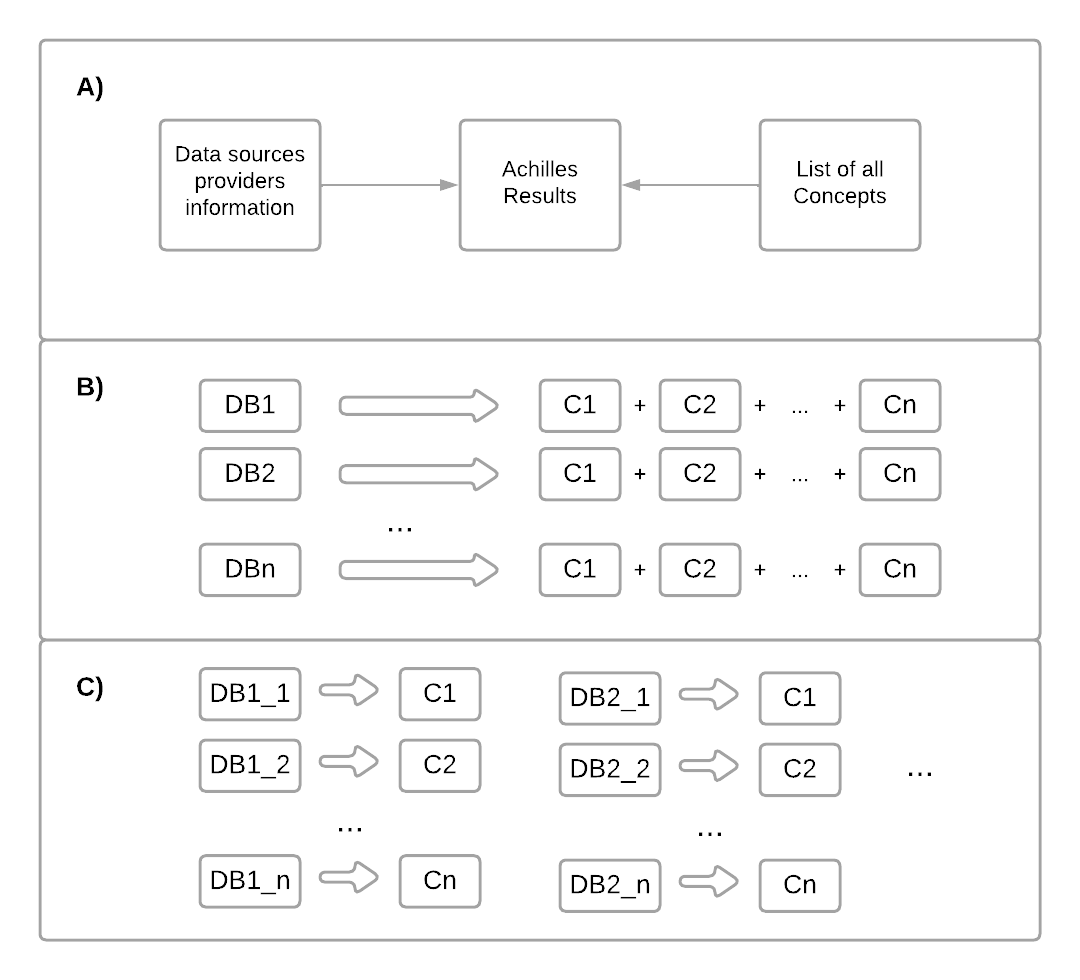
\includegraphics[width=0.8\textwidth]{figs/chapter3/index_struct.png}
    \centering
    \caption{Index data structure: A) All information about the databases is composed of three files, B) First approach to the structure of indexed documents, C) Current approach to the structure of indexed documents.}
    \label{fig_struct}
\end{figure}


The first approach to structure of the documents to be indexed is shown in Figure \ref{fig_struct}, part B). The document structure consists of a pairing of database IDs with their corresponding content. The content is represented as a single string, where each concept from each database is concatenated and separated by spaces. However, this way of indexing the database contents leads to unsatisfactory results of search.

\hl{TODO: explicar o porquê @tiago help :')}

The approach to creating the document structure has been refined to enhance the granularity and searchability of the database content. Each concept in the database is individually indexed, as shown in Figure~\ref{fig_struct}, part C). Each concept within a database is treated as a separate document for indexing purposes. This is achieved by assigning a document number (docno) that uniquely combines the database ID and the concept's position within its list. The 'docno' serves as a unique identifier for each concept, ensuring that each piece of data can be individually retrieved and queried. The content of each document, represented by the concept itself, is indexed under the text field. This allows for direct searching of concepts within the database, facilitating more precise and efficient retrieval of information. 


\subsubsection{Database Searching Process}
\label{searchprocess}

When the IR system receives a query in free text, the system processes it using Natural Language Processing (NLP) techniques applied to the query to enhance the search performance. These processes can include tokenization (splitting the text into individual terms or words), stemming or lemmatization (reducing words to their base form), and stop-word removal (eliminating common words that do not contribute to the search). Standardizing the text and transforming the query into important terms improves the match between the queries and indexed concepts as documents.

After processing the query, the BM25 algorithm evaluates the relevance of each concept within the database to the query, assigning a score that reflects its relevance. The method returns the 100 most relevant results and scores each concept. Then, these concepts are grouped by databases. The total relevance score for each database is calculated by summing the scores of its concepts. This comprehensive compilation process highlights the most relevant concepts. To ensure that only the most pertinent databases are presented to the user, the engine applies a predefined threshold to filter out databases with lower cumulative scores. The remaining results are then sorted in descending order of their total scores, prioritizing those with the highest relevance to the query.

Each element in the ranked list of databases contains the following information about the databases: a unique numeric identifier, the database name, the hash that identifies the database to be added to the link to access in the EHDEN Catalogue, the total relevance score assigned by the BM25 algorithm, indicating how well the database matches the query, and the concepts list that has been identified.


\subsection{API-driven Approach}

This project's Information Retrieval (IR) component is accessible through an API, allowing seamless integration with external systems. By exposing the endpoints of the IR component, the API facilitates the consumption of search functionalities, ensuring that various external applications can interact with the data effectively.

The API offers endpoints for submitting queries and retrieving search results. When a query is sent to the API, it undergoes the same searching steps described in the previous section (\ref{searchprocess}).

This API-driven approach enhances the IR component's interoperability and ensures that external systems can seamlessly query and retrieve data. This enables efficient and precise identification of the most suitable databases for any given query, facilitating the integration of the IR component in the following project implementation steps.


\section{Frameworks to streamline biomedical data discovery\protect\footnote{This section is mainly based in the publication \textit{Using Flowise to Streamline Biomedical Data Discovery and Analysis, IEEE 22nd Mediterranean Electrotechnical Conference (MELECON), 2024}}}

% tbd: overview de frameworks e como podem ser uteis
To achieve the proposed goal of making a conversational search assistant, a LLM has a crucial role in generating coherent, contextually relevant text and engaging in human language interactions. The LLM used in this project is \texttt{Nous Hermes 2 Mixtral 8x7B} open model. This model belongs to the llama family and has a 47B of parameters. The reason for using this LLM model is that it is a promising model, and the IEETA has installed it for use in its projects.

The LLM is installed a local version of the Ollama framework and deployed in a Virtual Machine to access the LLM using a URL. So, there are some options to integrate the model in the system. Flowise and Langflow are frameworks that enable build an LLM system without worrying with the orchestration flow between components. An overview of these frameworks and, in the case of Flowise, an implementation are presented below.


\subsection{Flowise}

Flowise\footnote{\url{https://github.com/FlowiseAI/Flowise}}, an open-source automation tool, plays a pivotal role by facilitating the integration of different Artificial Intelligence (AI) components, combined with IR techniques, as \citet{reis2024flowise} stated.

Flowise enables the creation of customized orchestration flows for Large Language Models (LLM) with AI agents and other tools. The workflows within Flowise consist of interconnected nodes or blocks that represent various actions or operations. The specific workflow implemented is illustrated in Figure~\ref{fig_workflow}.

\begin{figure*}[ht]
    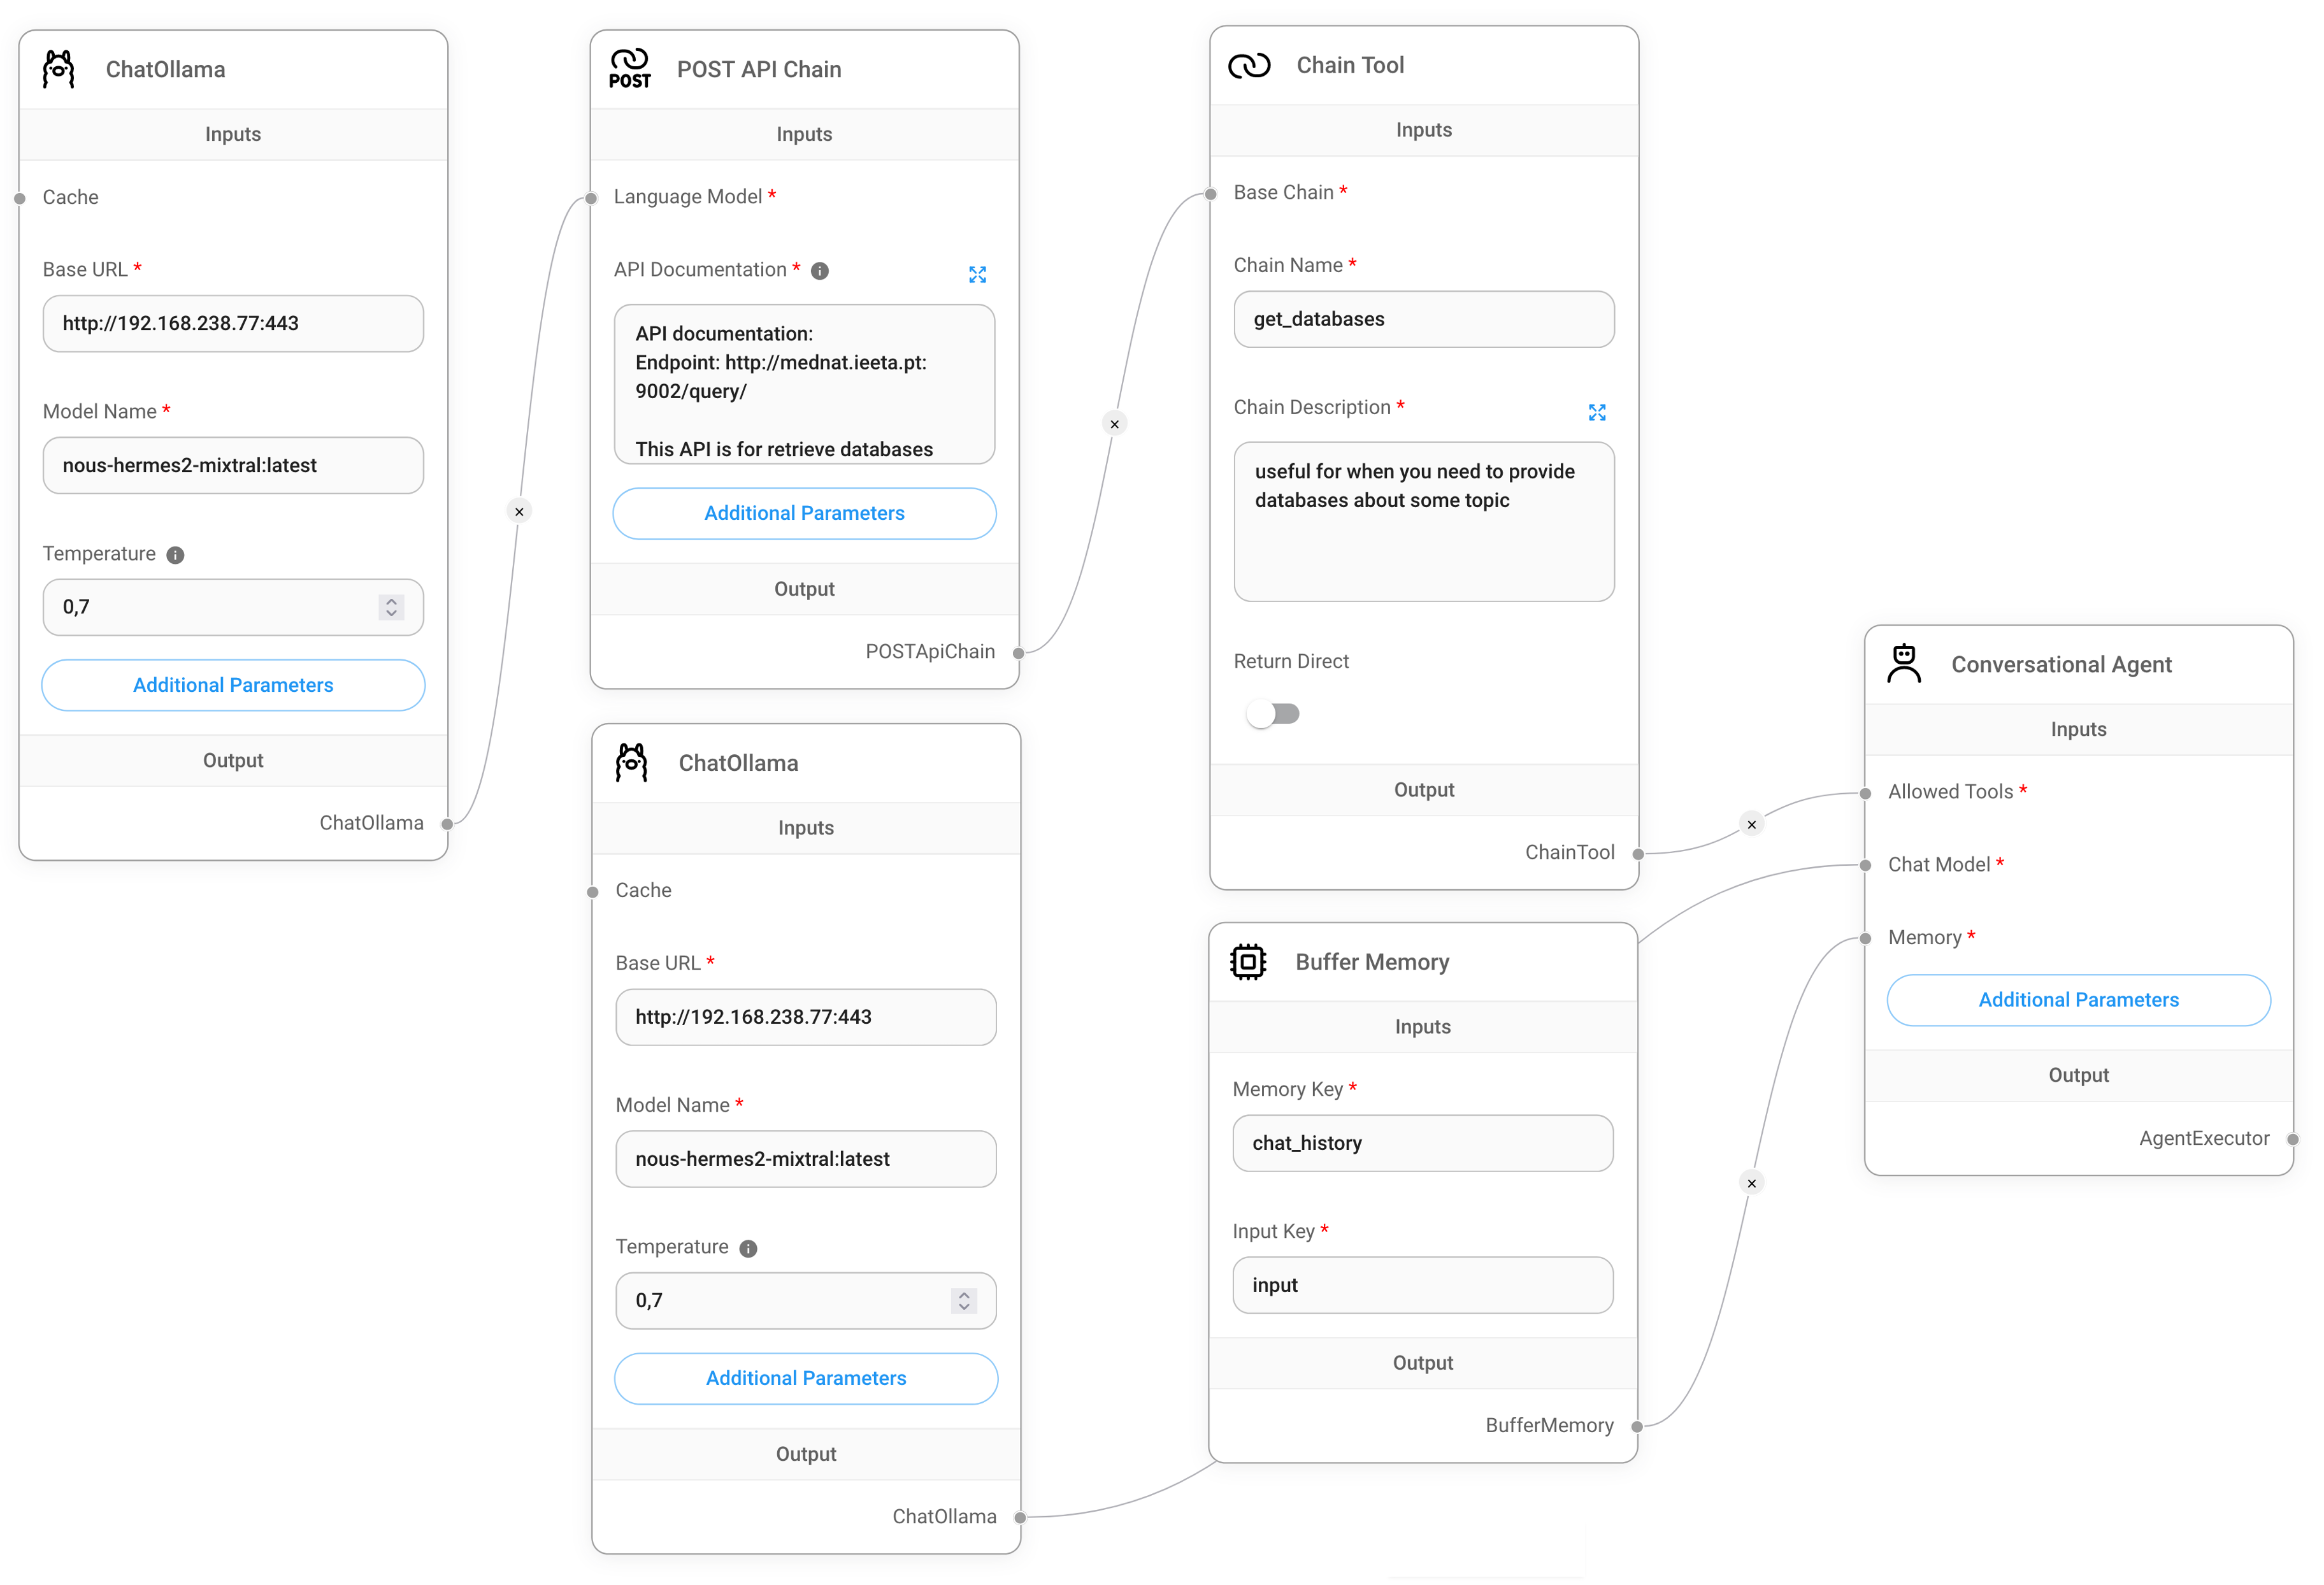
\includegraphics[width=1\textwidth]{figs/chapter3/workflow.png}
    \centering
    \caption{Worflow implemented in Flowise tool.}
    \label{fig_workflow}
\end{figure*}

The conversational agent employs a comprehensive approach to enable dynamic interactions on a healthcare information retrieval platform. It orchestrates the dialogue flow through the Conversational Agent Node, utilizing an LLM to provide a coherent and context-aware user experience. This node is configured with parameters that control tool access, chat model specifications, and memory capabilities, allowing it to maintain context or state information across interactions for structured conversations.

The core of conversational dynamics is powered by the ChatOllama Node, a chatbot engine designed for processing user queries and the generation of relevant responses. The implementation rely on Ollama\footnote{\url{https://ollama.com/}} since other solutions like ChatGPT API possess privacy issues. The Ollama operates based on a set of parameters including a base URL, alongside model specifications and a temperature setting that modulates probabilistic distribution over the predicted tokens. Furthermore, the Conversational Agent incorporates a Buffer Memory component, essential for the retention of interaction histories and stateful data. This component ensures the persistence of conversational context, a critical feature for enhancing user engagement and response relevance.

To provide the most relevant medical databases, a Retrieval-Augmented Generation~(RAG) architecture was adopted, as detailed in the section \ref{rag_section}. This approach applied to this scenario involves retrieving the best databases from the IR component and adding them to the LLM prompt. RAG enables the LLM to have up-to-date, valid, and domain-specific information to enhance response accuracy and relevance. 

The integration with the Chain Tool facilitates the application of prompt engineering techniques, enabling the agent to access the list of the recommended best databases. The tool consumes the endpoint of the IR component, which is better described in the section \ref{bm25implementation}. The conversational agent is equipped with real-time, accurate database recommendations, enhancing the quality of information provided to the user. 


\subsection{Langflow}

Langflow\footnote{\url{https://github.com/langflow-ai/langflow}} is another open-source tool to build AI applications. It is also a low-code tool that allows the integration of LLM and AI components. This tool simplifies the process of creating flows, such as chatflows. Users can drag components from the sidebar onto the canvas and connect them to begin building their applications. The platform allows for exploration by editing prompt parameters, grouping components into high-level components, and creating custom components. This intuitive interface makes Langflow a powerful tool for developing LLM-based applications.

% tbd: o que meto mais? não tenho implementação




\section{EHDEN Chatbot\protect\footnote{This section is mainly based in the publication \textit{A chatbot-like platform to enhance the
discovery of OMOP CDM databases, 34th Medical Informatics Europe Conference (MIE), 2024}}}


The system was designed to be integrated as a tool in the EHDEN Portal. Therefore, authentication issues were solved by the current mechanisms available on this platform~\cite{almeida2024federated}. Therefore, the system was implemented to use the MONTRA2-SDK~\cite{almeida2024montra2}. This also provided an interface to show the metadata, when researchers want to get more details about the suggested databases. 

Figure~\ref{fig_arch} represents the key components of the system and their interconnections. The Conversational User Interface~(UI) is the primary interface for user interaction, built on the React framework. The widget can be embedded into any web page or application with minimal coding effort. The UI records the user questions and conveys them to the backend to be processed in the component dedicated to IR. In different work, we tried to adopt an open-source automation tool to build Chatbot applications~\cite{reis2024flowise}. However, these become limited to address the new requirements. Therefore, FlowiseAI was replaced by a Python-based backend, developed for this system.

\begin{figure}[ht]
    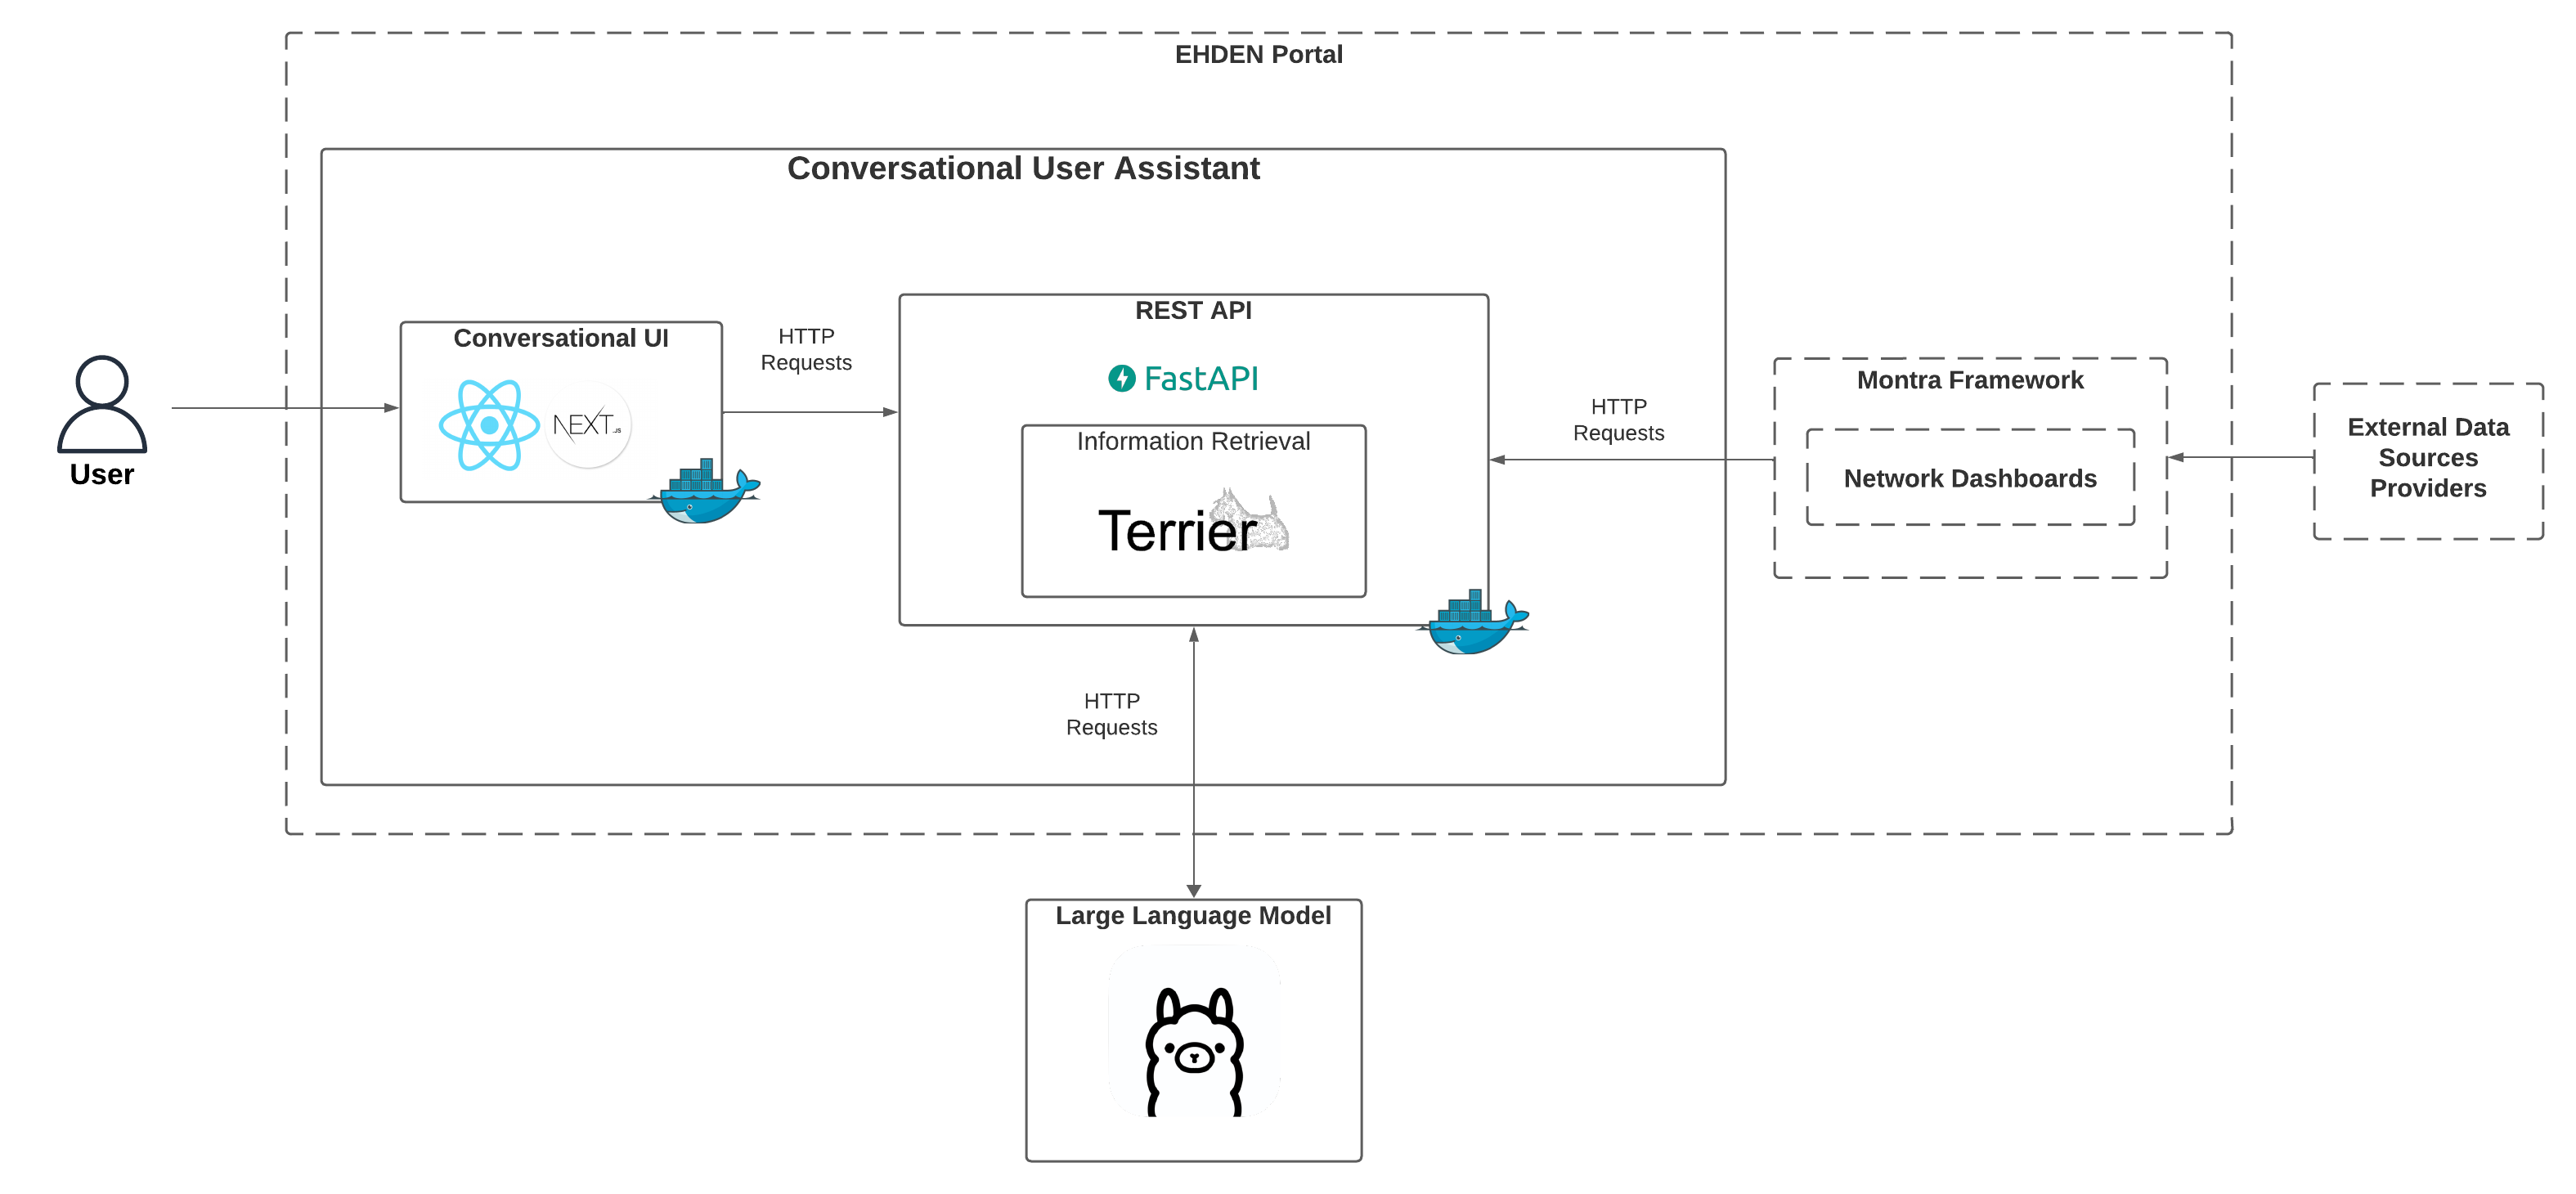
\includegraphics[width=\textwidth]{figs/chapter3/architecture.png}
    \centering
    \caption{Overview of the system architecture.}
    \label{fig_arch}
\end{figure}
